
\documentclass[t,8pt]{beamer}

\usepackage{graphicx,comment,amssymb,hyperref,array,longtable,tabularx,booktabs,ulem}
\usetheme{Pittsburgh}
\usecolortheme{crane}
\usepackage{xcolor}
\author{Dmitry Khovratovich }
\institute{ Ethereum Foundation }
\newtheorem{remark}{Remark}
\newtheorem{proposition}{Proposition}
\newtheorem{challenge}{Challenge}

\title{Skipping Bounds and Bounty Program 2026}

\begin{document}
\maketitle

\begin{frame}{Recent attack}
    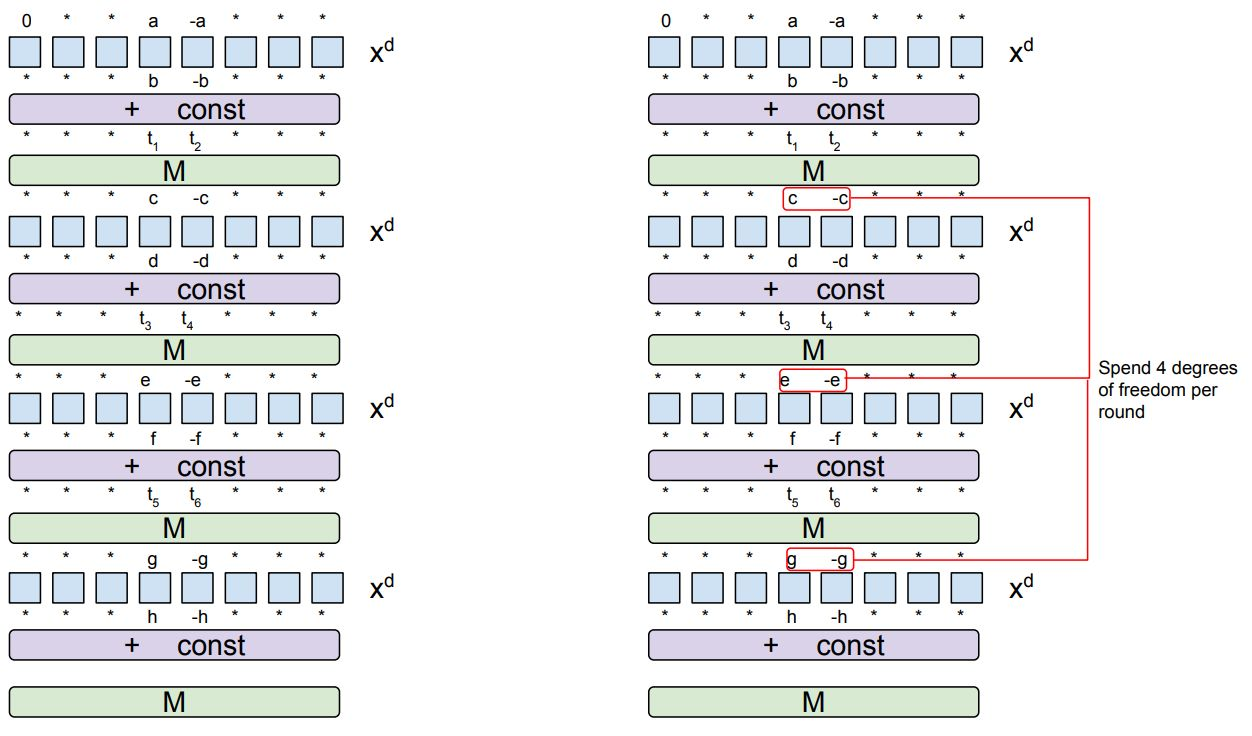
\includegraphics[width=\textwidth]{images/att1.jpg}
    By spending $4$ degrees of freedom per round, the attack
    can skip $\approx t/4$ full rounds of Poseidon2, effectively reducing the security margin by 4 rounds.

\end{frame}

\begin{frame}{Non-ideal diffusion exploited}
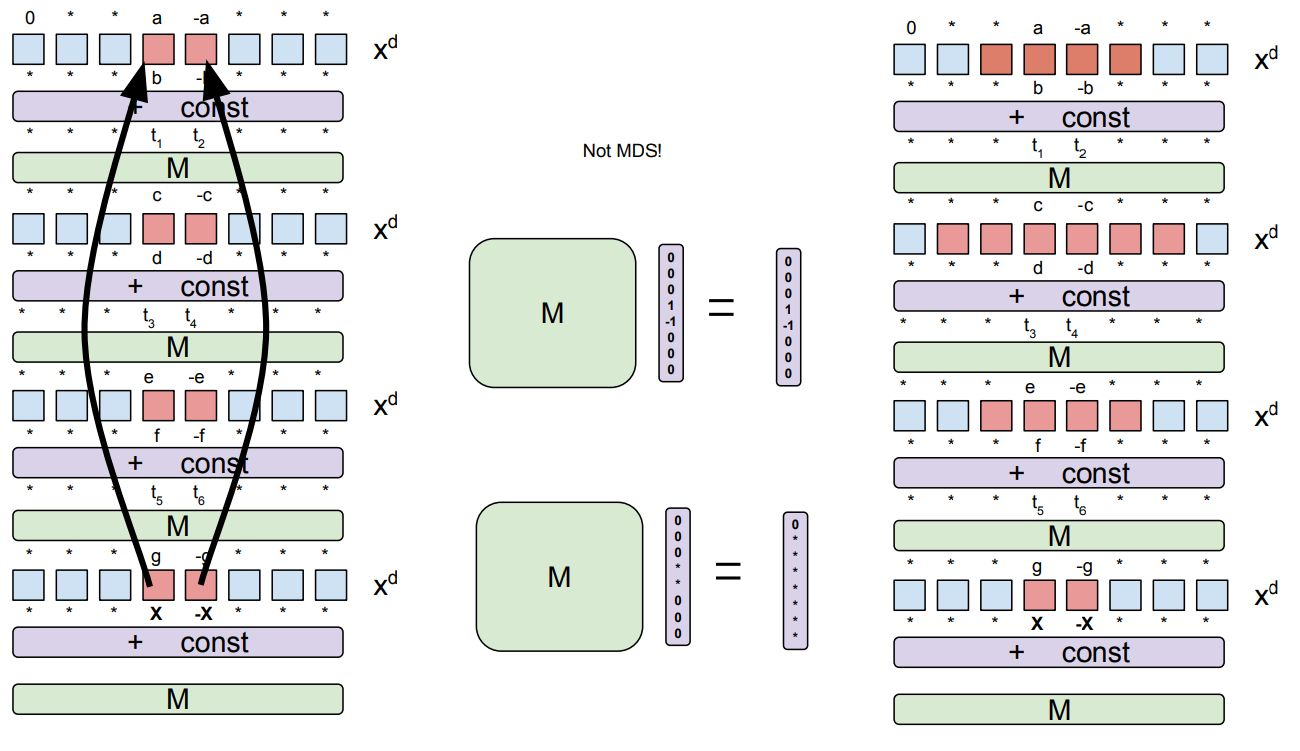
\includegraphics[width=\textwidth]{images/att2.jpg}
The attack exploits the specific structure of the linear layer with a certain high-probability
truncated differential.
\end{frame}

\begin{frame}{Upper bounds on the round number skipped}
 We show that all round skipping attacks reduce to two conditions:
 \begin{itemize}
        \item Existence of a truncated differential trail with few active S-boxes.
        \item  Existence of a sequence of states satisfying certain algebraic conditions (proportional
        to the number of active S-boxes).
    \end{itemize}
\begin{theorem}(Informal) A trail skipping $m$ rounds of an SPN structure with $t$ state elements
    and branch number $b$ must satisfy the following conditions:
    $$
    b\leq \frac{4t}{m},\text{ for } m \text{ even}  \qquad\qquad b\leq \frac{4t-2}{m-1},\text{ for } m \text{ odd}
    $$
\end{theorem}


\begin{proposition}
    If the linear transformation   is MDS, then a 4-round skipping trail cannot exist.
\end{proposition}

\begin{remark}
    Four rounds of an MDS-based SPN structure can potentially be skipped
    if the differential for the first round is relaxed.
\end{remark}

\end{frame}

\begin{frame}{Bounty program 2026}
   Bounty program consists of the following parts:
    \begin{itemize}
        \item CICO problem for round-reduced Poseidon1-KoalaBear;
        \item Density challenge (break as many rounds as possible);
        \item Zero-test challenge (break as many rounds as possible);
        \item Multi-target collision challenge (break as many rounds as possible);
        \item Ultimate prize: Partial Poseidon1 collisions. Collide on as many field elements as possible.
    \end{itemize}
\end{frame}


\begin{frame}{Density challenge}
    Parameters:
\begin{itemize}
    \item
\textbf{Attacked primitive:} hash function $H:\mathbb{F}_p^{*}\mapsto \mathbb{F}_p^{\ell}$.
\item
\textbf{Parameters:} $d,r,t\in\mathbb{Z}^{+}$ with condition $t\leq k\ell$.

\item \textbf{Decoding function:} $\mathrm{Decode}_{p,d}:\;\mathbb{F}_p\mapsto \mathbb{Z}_r^t$.
\end{itemize}
Challenge: find $S\in\mathbb{F}^r$ such that
\begin{align}
\#\{i:\,S[i]=0\}&\leq d\\
(a_0,a_1,\ldots,a_{\ell-1}) &:=H(S) \\
(i_0,i_1,\ldots,i_{k\ell-1})&:=\mathrm{Decode}(a_0)||\mathrm{Decode}(a_1)||\cdots||\mathrm{Decode}(a_{\ell-1})\\
S[i_j]&=0,\; j\in[t]
\end{align}
\end{frame}

\begin{frame}{Zero-test challenge}

\begin{itemize}
    \item
\textbf{Attacked primitive:} hash function $H:\mathbb{F}_p^{*}\mapsto \mathbb{F}_p^{\ell}$.
\item
\textbf{Parameters:} $d,r,t\in\mathbb{Z}^{+}$ with condition $t\leq \ell$.

\end{itemize}
Challenge: find multivariate polynomial  $P:\left(\mathbb{F}^r\right)^t\mapsto\mathbb{F}^r$ defined over the extension field $\mathbb{F}^r$ such that
\begin{align}
1\leq \mathrm{degree}(P)&\leq d\\
(a_0,a_1,\ldots,a_{\ell-1}) &:=H(\widehat{P}) \\
P(a_0,a_1, \ldots,a_{t-1})&=\mathbf{0}\in\mathbb{F}^r\label{eq:cond-zero}
\end{align}
where $\widehat{P}$ is the vector of the coefficients of $P$ expressed as elements of the base field $\mathbb{F}$. The length of  $\widehat{P}$ in the base field units is then $(d+1)r$.
\end{frame}

\begin{frame}{Partial collision challenge}

\begin{itemize}
    \item
\textbf{Attacked primitive:} hash function $H:\mathbb{F}_p^{*}\mapsto \mathbb{F}_p^{\ell}$.
\item
\textbf{Parameters:} $ t\in\mathbb{Z}^{+}$ with condition $t\leq \ell$.

Challenge: find $x\neq y\in\mathbb{F}^r$ such that
\begin{align}
(a_0,a_1,\ldots,a_{\ell-1}) &:=H(x) \\
(b_0,b_1,\ldots,b_{\ell-1}) &:=H(y) \\
a_i &= b_i ,\; i=0,1,\ldots,t-1.
\end{align}

\end{itemize}

\end{frame}

\end{document}